% -*- root: ../../DAT2-A423_Project_Report.tex -*-
\subsection{Implementation}
\label{sec:lsb-implementation}

The code for this programme can be seen in Appendix \ref{app:A}, and the algorithm we have implemented can be seen in Procedure \ref{alg1}.

By storing the information we want concealed in the two least significant bits, we can keep all of the message's original information, and changing each pixel of the cover image, by a maximum value of 3 or $00000011_2$, the concealed image will be almost invisible to the naked eye.

To do this, we had to make some restrictions on how big the cover image could be relative to the message image.
To not cause corruption and to ensure all information got saved, the cover image has to be four times as big as the hidden image, more specifically twice its height, and twice its width.
Each pixel of the concealed image will be stored within four pixels of the cover image, each masked differently, hence the size requirements.
We do this to get as much of the concealed image's information stored within the cover as possible.

To make both images easier to work with, we store each pixel's colour in their own array of type \lstinline|Color|.
To store each pixel within the cover, we first mask the cover to remove the information stored within the least significant bits, using the bitwise operator \&.
We then mask the concealed image to only keep the information stored in two bits, then right-shift those bits so the result will be a byte where only the least-significant-bits, can be 1, and then, add this information to the cover.
The result will be a pixel with its value for the Red, Green and Blue channels slightly changed by a value between 0 and 3.
The first pixel in the cover will contain the two most significant bits of the concealed image, the next will contain the third and fourth, and so on.

To recover the message image, we once again use the bitwise \& operator to only keep the information within the two least-significant bits of every pixel, then left-shift them accordingly and save this to a \lstinline|Color| array.
Once every pixel has been read, the \lstinline|Color| array can be transformed into an image which looks just like the original.

The entire process of encoding one pixel into four others using the two least significant bits is shown in figure \ref{fig:hundigrafik}.
We have the cover image $C$, the message image $M$ and the steganographic image $S$.
Each pixel in the message image is split up into four parts $M_1, M_2, M_3$ and $M_4$ where each part contains two bits from the R, G and B channels of the original pixel.

For every pixel chosen in $M$, four pixels are chosen from $C$.
For each of these pixels, we store the 6 most significant bits from the R, G and B channels in $C_1, C_2, C_3$ and $C_4$.

Lastly, four pixels in $S$ are created by making pairs in the form of $C_nM_n$.
This means that the four pixels in $S$ will be the following combinations: $C_1M_1,C_2M_2,C_3M_3$ and $C_4M_4$.

\begin{figure}
	\centering
	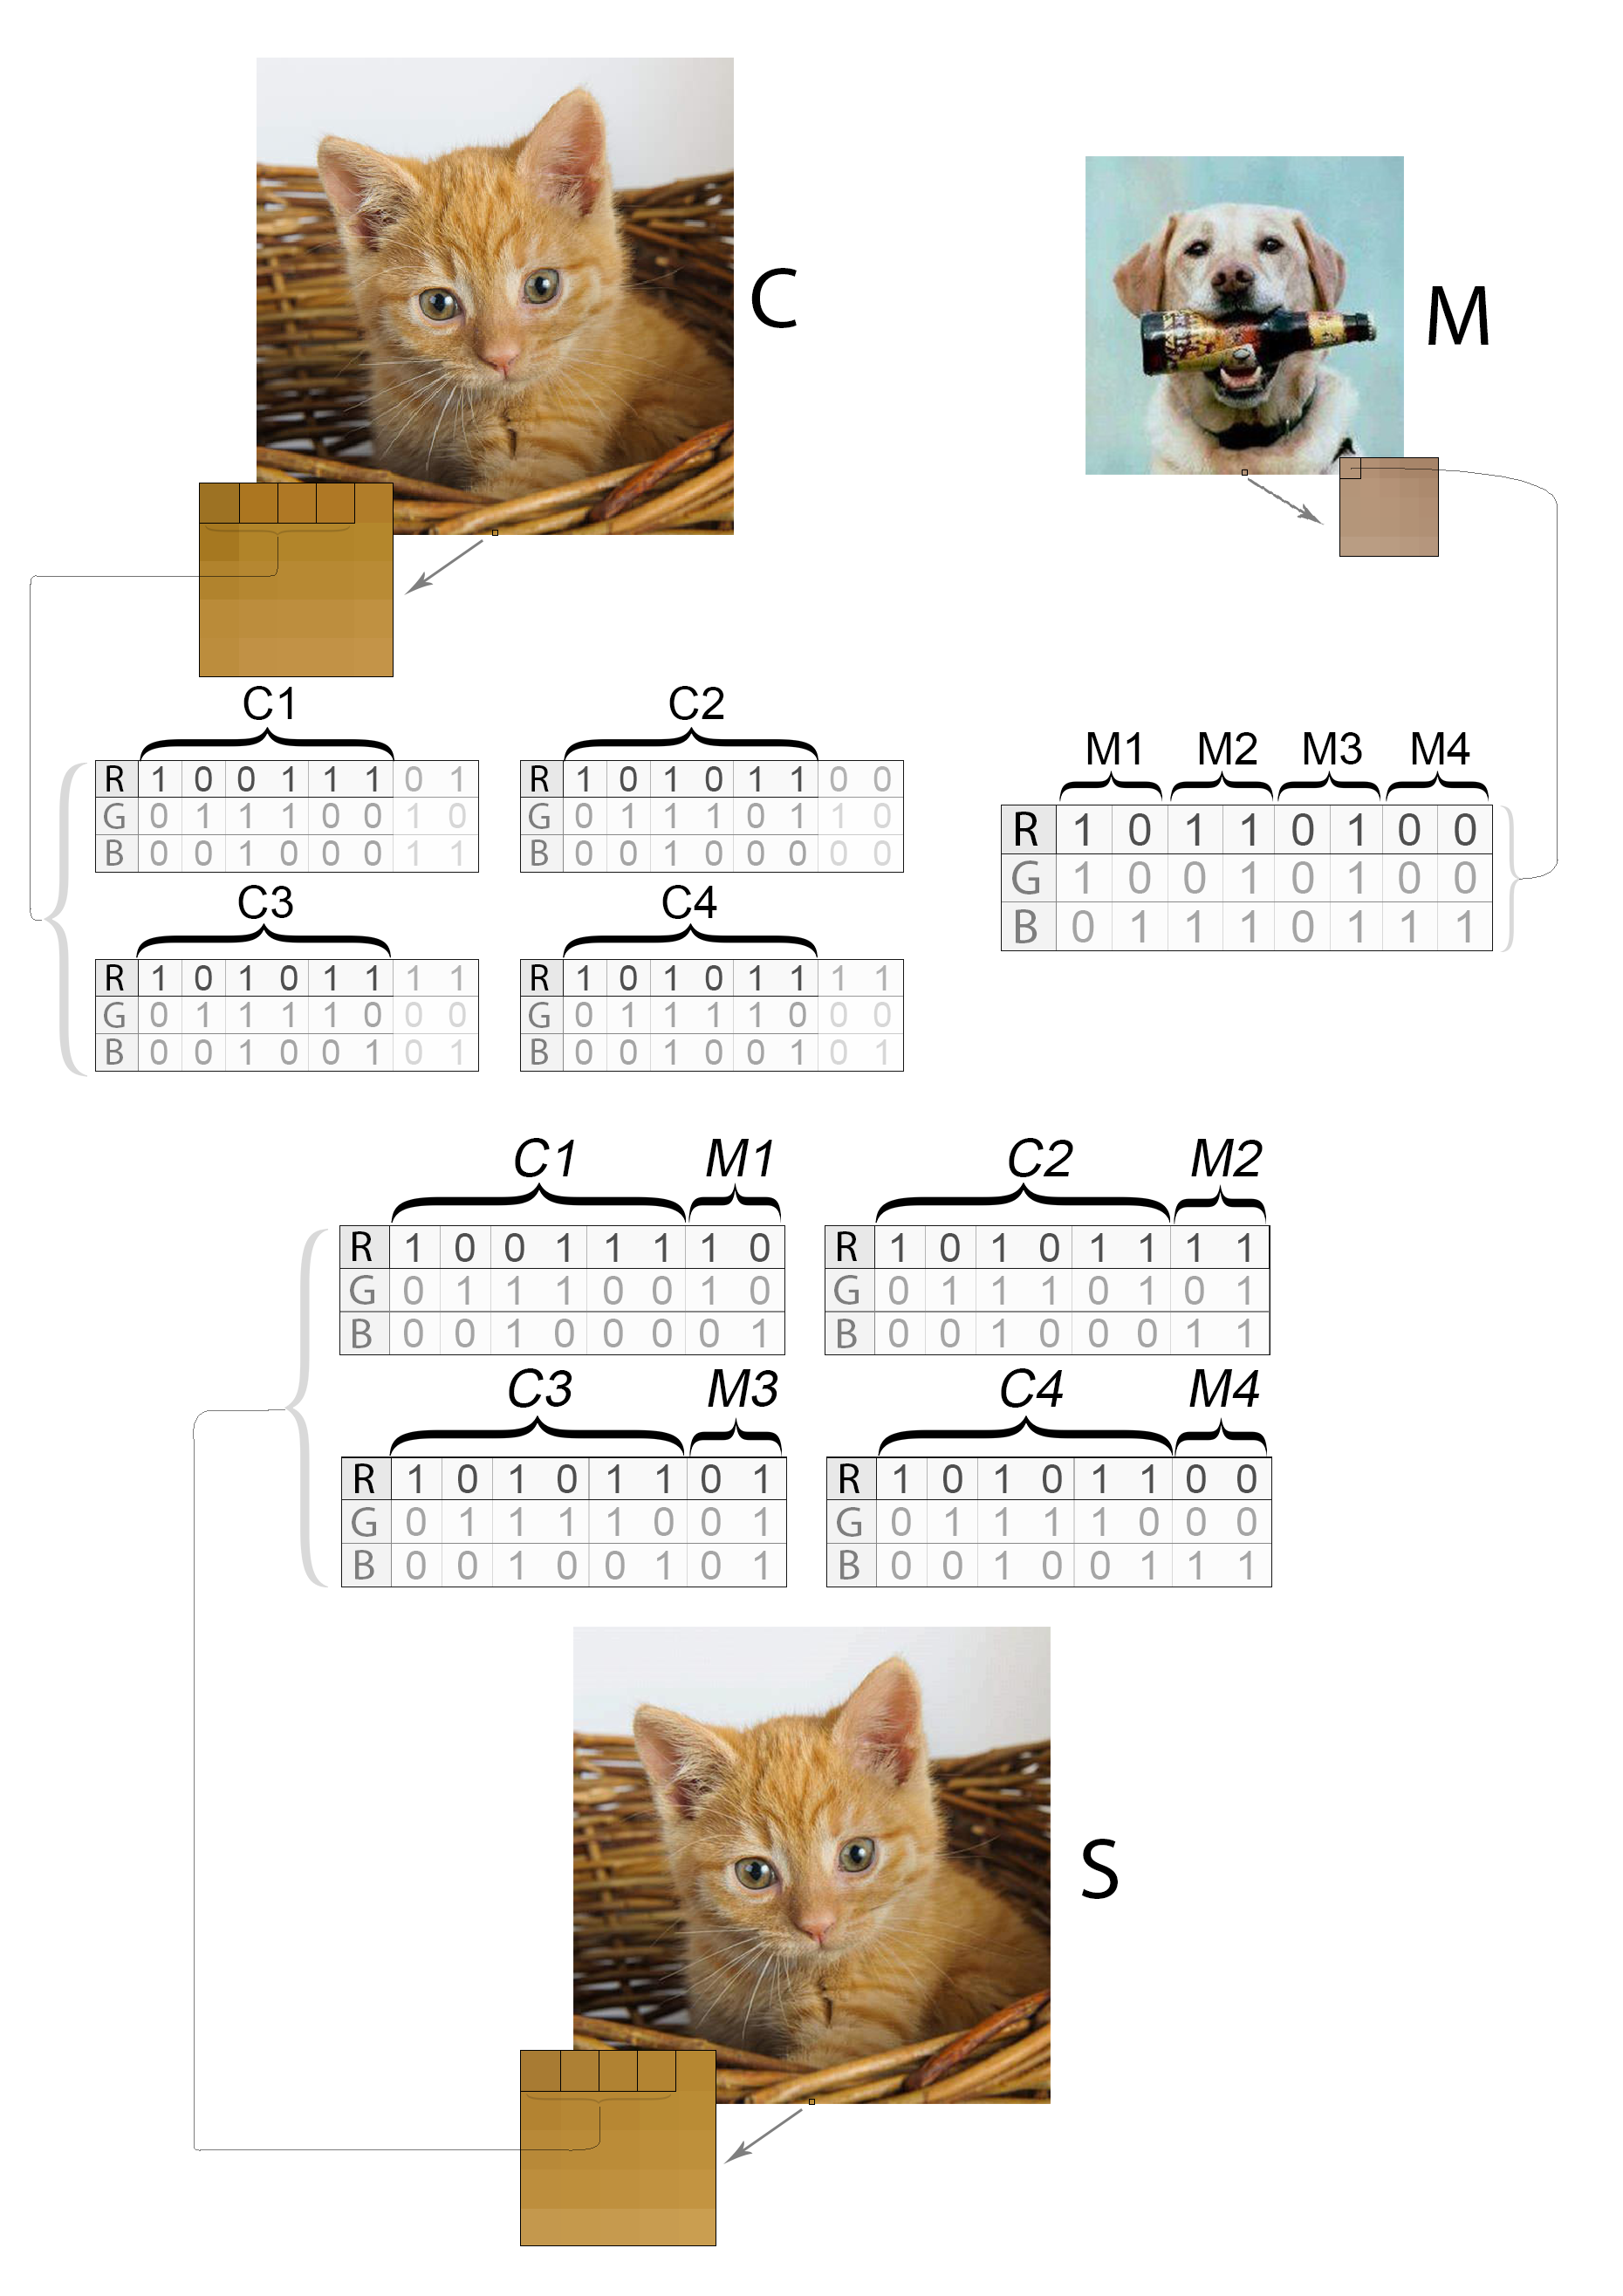
\includegraphics[width=1\textwidth]{figures/hundikatgrafik.png}
	\caption{Illustration of how the message is saved within its cover image.}
	\label{fig:hundigrafik}
\end{figure}

% -*- root: ../../DAT2-A423_Project_Report.tex -*-
\begin{algorithm}
\caption{Using the Two Least Significant Bits for Storing Data in an Image}
\label{alg1}
\begin{algorithmic}
\REQUIRE True-color bitmap images $c = \{c_1,c_2\ldots c_{WH}\}$ with size $W \times H$ where $c_{xW+y}$ is the pixel at location $(x,y)$ and $m  = \{m_1,m_2\ldots m_{\frac{WH}{4}}\}$ with size $\frac{W}{2} \times \frac{H}{2}$ where $m_{xW/2+y}$ is the pixel at location $(x,y)$
\ENSURE True-color bitmap image $s  = \{s_1,s_2\ldots s_{WH}\}$ of size $W \times H$ and where $s_{xW+y}$ is the pixel at location $(x,y)$ and where $m$ is embedded in $c$

\STATE{$k := 1$}
\FOR {$i:=1$ \TO $i=\frac{WH}{4}$}
	\FOR {$j:=1$ \TO $j=4$}
		\STATE{Set the first 6 bits in the R, G and B bytes $k$th element of $s$ to be the first 6 bits of the R, G and B bytes of the $k$th element of $c$}

		\STATE{Set the 7th bit in the R, G and B bytes in the $k$th element of $s$ with the $(j\cdot 2 - 1)$th bit in the R, G and B bytes in the $i$th element in $m$}

		\STATE{Set the 8th bit in the R, G and B bytes in the $k$th element of $s$ with the $(j\cdot 2)$th bit in the R, G and B bytes in the $i$th element in $m$}

		\STATE{$k := k + 1$}
	\ENDFOR
\ENDFOR

\RETURN $s$
\end{algorithmic}
\end{algorithm}

\subsection*{Conclusion}
We now have an understanding of how basic steganography with the LSB-method works. This knowledge will help us understand other methods used in steganography, as well as help us develop a product using a method that is not as easily compromised as this implementation is.